\documentclass[twoside,11pt,a4paper]{report}
\usepackage[utf8]{inputenc}
%colorarea celulelor din tabele
\usepackage[table]{xcolor}
%pentru simboluri
%\usepackage{amssymb}
%comanda thead din tabele
\usepackage{makecell}
%combinarea randurilor unui tabel
\usepackage{multirow}
%linierea a unor celule specifice 
\usepackage{hhline}
%inserarea imaginilor 
\usepackage{graphicx}
%crearea header-ului
\usepackage{fancyhdr}
%aliniearea textului
\usepackage{ragged2e}
%crearea referintelor catre o imagine/tabel
\usepackage{hyperref}
%controlarea spatieri intre randuri in diverse situatii
\usepackage[nodisplayskipstretch]{setspace}
%schimbarea formatului titlurilor
\usepackage{titlesec}
\titleformat{\chapter}{\normalfont\huge\bfseries}{\thechapter.}{16pt}{\huge}
\titlespacing{\chapter}{0cm}{0cm}{0cm}
%font
\usepackage{newtxtext,newtxmath}

%alinierea
\usepackage[top=2.5cm, bottom=2cm, left=2.5cm, right=2cm]{geometry}
%\setlength{\headheight}{-1.50cm}
\setlength{\headsep}{0.50cm}

%setare path catre imagini
\graphicspath{{continut/imagini}}
\pagenumbering{roman}
%setare header
\renewcommand{\headrulewidth}{0pt} %pt a elimina linia de sub header
\fancyhf{}
\rfoot{\begin{center}\thepage \end{center}}
\renewcommand{\figurename}{\textbf{Figura}}
\renewcommand{\thefigure}{\textbf{\arabic{figure}}}

\renewcommand{\tablename}{\textbf{Tabelul}}
\renewcommand{\thetable}{\textbf{\arabic{table}}}

\renewcommand{\contentsname}{CUPRINSUL}
\renewcommand{\listfigurename}{LISTA FIGURILOR}
\renewcommand{\listtablename}{LISTA TABELELOR}

\begin{document}

\thispagestyle{fancy}
\pagenumbering{gobble}

\fancyhead[LE,RO]{

\includegraphics[scale=0.7]{icon2.png}}

\fancyhead[RE,LO]{

\includegraphics[scale=0.5]{icon1.png}
}

%mijlocul headerului
\fancyhead[CE,CO]{
    \fontsize{10}{11}\selectfont
    UNIVERSITATEA DIN CRAIOVA \\
FACULTATEA DE AUTOMATICĂ, CALCULATOARE ȘI \\
ELECTRONICĂ \\~\\
DEPARTAMENTUL DE \textcolor{red}{[CALCULATOARE ȘI TEHNOLOGIA \\
INFORMAȚIEI / AUTOMATICĂ ȘI ELECTRONICĂ / MECATRONICĂ\\
ȘI ROBOTICĂ]}
}

\phantom{.}
\\[18\baselineskip]
\begin{center}
    \fontsize{14}{11}\selectfont
PROIECT DE DIPLOMĂ
\\[2\baselineskip]
\textcolor{red}{[\textit{Prenumele și numele candidatului}]}
\\[10\baselineskip]
\fontsize{12}{11}\selectfont
COORDONATOR ȘTIINȚIFIC
\\[2\baselineskip]
\textcolor{red}{[\textit{Titlul științific, prenumele și numele coordonatorului}]}
\\[19\baselineskip]
\textcolor{red}{[\textit{Luna (în litere) și anul susținerii proiectului}]}\\~\\
CRAIOVA
\end{center}

\newpage
\thispagestyle{fancy}
\pagenumbering{gobble}

\fancyhead[LE,RO]{

\includegraphics[scale=0.7]{icon2.png}}

\fancyhead[RE,LO]{

\includegraphics[scale=0.5]{icon1.png}
}

%mijlocul headerului
\fancyhead[CE,CO]{
    \fontsize{10}{11}\selectfont
    UNIVERSITATEA DIN CRAIOVA \\
FACULTATEA DE AUTOMATICĂ, CALCULATOARE ȘI \\
ELECTRONICĂ \\~\\
DEPARTAMENTUL DE \textcolor{red}{[CALCULATOARE ȘI TEHNOLOGIA \\
INFORMAȚIEI / AUTOMATICĂ ȘI ELECTRONICĂ / MECATRONICĂ\\
ȘI ROBOTICĂ]}
}


\phantom{.}
\\[19\baselineskip]
\begin{center}
    
    \fontsize{14}{11}\selectfont
\textcolor{red}{[\textit{TITLUL PROIECTULUI DE DIPLOMĂ}]}
\\[2\baselineskip]
\textcolor{red}{[\textit{Prenumele și numele candidatului}]}
\\[13\baselineskip]
\fontsize{12}{11}\selectfont
COORDONATOR ȘTIINȚIFIC
\\[2\baselineskip]
\textcolor{red}{[\textit{Titlul științific, prenumele și numele coordonatorului}]}
\\[13\baselineskip]
\textcolor{red}{[\textit{Luna (în litere) și anul susținerii proiectului}]}\\~\\~\\
CRAIOVA

\end{center}

\newpage
\pagenumbering{roman}
\setcounter{page}{3}

\begin{flushright}
    \phantom{.}
    \\[3\baselineskip]
    \textit{,,Învățătura este o comoară care își urmează stăpânul pretutindeni.''}\\~\\
Proverb popular
\end{flushright}


\newpage
\begin{center}
    \fontsize{12}{11}\selectfont
    \textbf{DECLARAȚIE DE ORIGINALITATE}
    \\[4\baselineskip]
    \end{center}
    
    \renewcommand{\baselinestretch}{1.8}
    \raggedright
        \fontsize{11}{11}\selectfont
    Subsemnatul \textcolor{red}{[\textit{PRENUMELE ȘI NUMELE CANDIDATULUI}]}, student la specializarea \textcolor{red}{[\textit{DENUMIREA OFICIALĂ 
    A SPECIALIZĂRII}]} din cadrul Facultății de Automatică, Calculatoare și Electronică a Universității din Craiova, certific prin 
    prezenta că am luat la cunoştinţă de cele prezentate mai jos şi că îmi asum, în acest context, originalitatea 
    proiectului meu de licenţă: 
        \begin{itemize}
            \setlength\itemsep{-0.5em}
            \item cu titlul \textcolor{red}{[\textit{TITLUL LUCRĂRII}]}, 
            \item coordonată de \textcolor{red}{[\textit{TITLUL ȘTIINȚIFIC, PRENUMELE ȘI NUMELE COORDONATORULUI}]}, 
            \item prezentată în sesiunea \textcolor{red}{[\textit{LUNA ȘI ANUL SESIUNII DE LICENȚĂ}]}.
        \end{itemize}
    
        La elaborarea proiectului de licenţă, se consideră plagiat una dintre următoarele acţiuni: 
        \begin{itemize}
            \setlength\itemsep{-0.5em}
            \item reproducerea exactă a cuvintelor unui alt autor, dintr-o altă lucrare, în limba română sau prin traducere dintr-o altă limbă, dacă se omit ghilimele şi referinţa precisă, 
            \item redarea cu alte cuvinte, reformularea prin cuvinte proprii sau rezumarea ideilor din alte lucrări, dacă nu se indică sursa bibliografică, 
            \item prezentarea unor date experimentale obţinute sau a unor aplicaţii realizate de alţi autori fără menţionarea corectă a acestor surse, 
            \item însuşirea totală sau parţială a unei lucrări în care regulile de mai sus sunt respectate, dar care are alt autor. 
        \end{itemize}
        Pentru evitarea acestor situaţii neplăcute se recomandă:
        \begin{itemize}
            \setlength\itemsep{-0.5em}
            \item plasarea între ghilimele a citatelor directe şi indicarea referinţei într-o listă corespunzătoare la sfărşitul lucrării, 
            \item indicarea în text a reformulării unei idei, opinii sau teorii şi corespunzător în lista de referinţe a sursei originale de la care s-a făcut preluarea, 
            \item precizarea sursei de la care s-au preluat date experimentale, descrieri tehnice, figuri, imagini, statistici, tabele et caetera, 
            \item precizarea referinţelor poate fi omisă dacă se folosesc informaţii sau teorii arhicunoscute, a căror paternitate este unanim cunoscută și acceptată.
        \end{itemize}
        Data,  \hfill Semnătura candidatului, 

\newpage
\begin{singlespace}
    \begin{minipage}[t]{0.1\textwidth}
        \phantom{.}
        \\[-0.8\baselineskip]
        
\includegraphics[width=\linewidth]{icon2.png}
    \end{minipage}%
    \hfill
    \begin{minipage}[t]{0.6\textwidth}\raggedright
        UNIVERSITATEA DIN CRAIOVA\\
        Facultatea de Automatică, Calculatoare şi Electronică\\~\\
        Departamentul de \textcolor{red}{[Calculatoare și Tehnologia Informației / \\
        Automatică și Electronică / Mecatronică și Robotică]}
    \end{minipage}%
    \hfill
    \begin{minipage}[t]{0.2\textwidth}\begin{center}
        \fontsize{10}{11}\selectfont
        \phantom{.}
        Aprobat la data de\\
        …………………\\
        Şef de departament,\\
        Prof. dr. ing.\\ \textcolor{red}{Marius BREZOVAN/\\Comin IONETE/\\Dorian COJOCARU}
\end{center}\end{minipage}\end{singlespace}

\begin{center}
    \textbf{PROIECTUL DE DIPLOMĂ}
\end{center}

\begin{center}
\begin{singlespace}
\renewcommand{\arraystretch}{2.5}
    \begin{tabular}{ |p{5.9cm}|p{10cm}| } 

    \hline\cellcolor[HTML]{f2f2f2}
    \begin{center}Numele și prenumele studentului/-ei:\end{center} &  \\ 
    \hline\cellcolor[HTML]{f2f2f2}
    \begin{center}Enunțul temei:\end{center} & \textcolor{red}{[\textit{Titlul lucrării / descrierea pe scurt a temei}]}  \\ 
    \hline\cellcolor[HTML]{f2f2f2}
    \begin{center}Datele de pornire:\end{center} & \textcolor{red}{[\textit{Descrierea datelor inițiale de la care s-a început activitatea de cercetare/dezvoltare a tezei}]} \\ 
    \hline\cellcolor[HTML]{f2f2f2}
    \begin{center}Conținutul proiectului::\end{center} & \textcolor{red}{[\textit{Descrierea succintă a conținutului fiecărui capitol al lucrării}]} \\
    \hline\cellcolor[HTML]{f2f2f2}
    \begin{center}Material grafic obligatoriu:\end{center} &  \\
    \hline\cellcolor[HTML]{f2f2f2}
    \begin{center}Consultații:\end{center} & \textcolor{red}{[\textit{Periodice/zilnice/săptămânale/lunare}]} \\
    \hline\cellcolor[HTML]{f2f2f2}
    \begin{center}Conducătorul științific\\
    (titlul, nume și prenume, semnătura):
    \end{center} & \textcolor{red}{Șef lucrări dr. ing. Marius MARIAN} \\
    \hline

    \end{tabular}
        
\newpage
\renewcommand{\arraystretch}{0.1}
    \begin{tabular}{ |p{5.9cm}|p{10cm}| }

    \hline\cellcolor[HTML]{f2f2f2}
    \begin{center}Data eliberării temei:\end{center} & \begin{center}\textcolor{red}{15.10.2021}\end{center} \\
    \hline\cellcolor[HTML]{f2f2f2}
    \begin{center}Termenul estimat de predare a proiectului:\end{center} & \begin{center}\textcolor{red}{01.06.2022}\end{center} \\
    \hline\cellcolor[HTML]{f2f2f2}
    \begin{center}Data predării proiectului de către\\ student și semnătura acestuia:\end{center} &  \\
    \hline

    \end{tabular}\end{singlespace}
\end{center}
\newpage
\begin{singlespace}
        
    \begin{minipage}{0.1\textwidth}   
        
\includegraphics[width=\linewidth]{icon2.png}
    \end{minipage}%
    \hfill
    \begin{minipage}{0.85\textwidth}\raggedright
        UNIVERSITATEA DIN CRAIOVA\\
        Facultatea de Automatică, Calculatoare şi Electronică\\~\\
        Departamentul de \textcolor{red}{[Calculatoare și Tehnologia Informației / \\
        Automatică și Electronică / Mecatronică și Robotică]} \\~\\
    \end{minipage}
\end{singlespace}
    
    \begin{center}
        \fontsize{12}{11}\selectfont
        \phantom{.}
        \\[1\baselineskip]
        \textbf{REFERATUL CONDUCĂTORULUI ȘTIINȚIFIC}
    \end{center}

    \begin{singlespace}
        \fontsize{11}{11}\selectfont
        \begin{minipage}{.4\textwidth}
            Numele și prenumele candidatului/-ei:\\
            Specializarea:\\
            Titlul proiectului: \\~\\
            Locația în care s-a realizat practica de documentare (se bifează una sau mai multe din opțiunile din dreapta):
          \end{minipage}\hfill
          \begin{minipage}{.55\textwidth}
            \phantom{.}
        \\[4\baselineskip]
            \textcolor{red}{[\textit{Denumirea oficială a specializării absolvite de candidat}]\\\relax
            [\textit{Titlul lucrării}]}\\~\\
            În facultate   \\~\\
            În producție  \\~\\
            În cercetare   \\~\\
            Altă locație:  \textcolor{red}{[\textit{se detaliază}]}

          \end{minipage}
          \\[3\baselineskip]
        În urma analizei lucrării candidatului au fost constatate următoarele:\\~\\
        
        \begin{center}
        \renewcommand{\arraystretch}{1.5}
        \begin{tabular}{ |c|c|c|c|c|} 
            \hline\cellcolor[HTML]{f2f2f2}\centering
                 Nivelul documentării & \thead{Insuficient\\~\\\scalebox{2}{$\square$}}  & \thead{Satisfăcător\\~\\\scalebox{2}{$\square$}}  & \thead{Bine\\~\\\scalebox{2}{$\square$}}  & \thead{Foarte bine\\~\\\scalebox{2}{$\square$}}  \\ 
            \hline\cellcolor[HTML]{f2f2f2}\centering
            Tipul proiectului & \thead{Cercetare  \\~\\\scalebox{2}{$\square$}}  & \thead{Proiectare  \\~\\\scalebox{2}{$\square$}}  & \thead{Realizare practică \\~\\\scalebox{2}{$\square$}}  & \thead{Altul \\~\\\relax\textcolor{red}{[\textit{se detaliază}]}} \\
            \hline\cellcolor[HTML]{f2f2f2}\centering
            Aparatul matematic utilizat & \thead{Simplu  \\~\\\scalebox{2}{$\square$}}  & \thead{Mediu  \\~\\\scalebox{2}{$\square$}}  & \thead{Complex  \\~\\\scalebox{2}{$\square$}}  & \thead{Absent\\~\\\scalebox{2}{$\square$}}   \\
            \hline\cellcolor[HTML]{f2f2f2}\centering
            Utilitate & \thead{Contract de cercetare  \\~\\\scalebox{2}{$\square$}}  & \thead{Cercetare internă  \\~\\\scalebox{2}{$\square$}}  & \thead{Utilare \\~\\\scalebox{2}{$\square$}}  & \thead{Altul \\~\\\relax\textcolor{red}{[\textit{se detaliază}]}}  \\
            \hline\cellcolor[HTML]{f2f2f2}\centering
            Redactarea lucrării & \thead{Insuficient\\~\\\scalebox{2}{$\square$}}  & \thead{Satisfăcător\\~\\\scalebox{2}{$\square$}}  & \thead{Bine\\~\\\scalebox{2}{$\square$}}  & \thead{Foarte bine\\~\\\scalebox{2}{$\square$}}   \\
            \hline\cellcolor[HTML]{f2f2f2}\centering
            Partea grafică, desene & \thead{Insuficientă\\~\\\scalebox{2}{$\square$}}  & \thead{Satisfăcător\\~\\\scalebox{2}{$\square$}}  & \thead{Bună\\~\\\scalebox{2}{$\square$}}  & \thead{Foarte bună  \\~\\\scalebox{2}{$\square$}}   \\
            \hline
           \end{tabular}
        \end{center}
    \end{singlespace}

    \newpage

    \begin{singlespace}
        \begin{center}
            \begin{tabular}{ |>{\columncolor[HTML]{f2f2f2}}c|>{\columncolor[HTML]{f2f2f2}}c|c|c|c|c|}
\hline\multirow{8}{*}{}   \thead{Realizarea \\ practică}    & Contribuția autorului & \thead{Insuficientă\\~\\\scalebox{2}{$\square$}}  & \thead{Satisfăcătoare\\~\\\scalebox{2}{$\square$}}  & \thead{Mare\\~\\\scalebox{2}{$\square$}}  & \thead{Foarte mare\\~\\\scalebox{2}{$\square$}} \\\hhline{~~----}
                                                            &Complexitatea temei & \thead{Simplă \\~\\\scalebox{2}{$\square$}}  & \thead{Medie\\~\\\scalebox{2}{$\square$}}  & \thead{Mare\\~\\\scalebox{2}{$\square$}}  & \thead{Complexă  \\~\\\scalebox{2}{$\square$}} \\\hhline{~~----}
                                                            & Analiza cerințelor & \thead{Insuficient\\~\\\scalebox{2}{$\square$}}  & \thead{Satisfăcător\\~\\\scalebox{2}{$\square$}}  & \thead{Bine\\~\\\scalebox{2}{$\square$}}  & \thead{Foarte bine\\~\\\scalebox{2}{$\square$}} \\\hhline{~~----}
                                                            & Arhitectura  & \thead{Simplă \\~\\\scalebox{2}{$\square$}}  & \thead{Medie\\~\\\scalebox{2}{$\square$}}  & \thead{Mare\\~\\\scalebox{2}{$\square$}}  & \thead{Complexă  \\~\\\scalebox{2}{$\square$}} \\\cline{2-6} 
                                                            & Întocmirea specificațiilor funcționale & \thead{Insuficientă\\~\\\scalebox{2}{$\square$}}  & \thead{Satisfăcătoare\\~\\\scalebox{2}{$\square$}}  & \thead{Bună\\~\\\scalebox{2}{$\square$}}  & \thead{Foarte bună  \\~\\\scalebox{2}{$\square$}}  \\\cline{2-6}
                                                            & Implementarea & \thead{Insuficientă\\~\\\scalebox{2}{$\square$}}  & \thead{Satisfăcătoare\\~\\\scalebox{2}{$\square$}}  & \thead{Bună\\~\\\scalebox{2}{$\square$}}  & \thead{Foarte bună  \\~\\\scalebox{2}{$\square$}}  \\\cline{2-6}
                                                            & Testarea & \thead{Insuficientă\\~\\\scalebox{2}{$\square$}}  & \thead{Satisfăcătoare\\~\\\scalebox{2}{$\square$}}  & \thead{Bună\\~\\\scalebox{2}{$\square$}}  & \thead{Foarte bună  \\~\\\scalebox{2}{$\square$}}  \\\cline{2-6}
                                                            & Funcționarea & \thead{Da\\~\\\scalebox{2}{$\square$}}  & \thead{Parțială\\~\\\scalebox{2}{$\square$}}  & \multicolumn{2}{c|}{\thead{Nu\\~\\\scalebox{2}{$\square$}}}   \\\hline
               \multicolumn{2}{|>{\columncolor[HTML]{f2f2f2}}c}{Rezultate experimentale} & \multicolumn{2}{|c}{\thead{Experiment propriu \\~\\\scalebox{2}{$\square$}}} & \multicolumn{2}{|c|}{\thead{Preluare din bibliografie  \\~\\\scalebox{2}{$\square$}}} \\\hline
               \multicolumn{2}{|>{\columncolor[HTML]{f2f2f2}}c|}{Bibliografie}           & \thead{Cărți\\\phantom{.}} & \thead{Reviste\\\phantom{.}}  & \thead{Articole\\\phantom{.}}  & \thead{Referințe web  \\\phantom{.}}   \\\hline
               \multicolumn{2}{|>{\columncolor[HTML]{f2f2f2}}c|}{Comentarii} & \multicolumn{4}{c|}{} \\
               \multicolumn{2}{|>{\columncolor[HTML]{f2f2f2}}c|}{și} & \multicolumn{4}{c|}{} \\
               \multicolumn{2}{|>{\columncolor[HTML]{f2f2f2}}c|}{observații} & \multicolumn{4}{c|}{} \\\hline
            \end{tabular}
        \end{center}
    \end{singlespace}

\newpage

\begin{center}
    \fontsize{16}{11}\selectfont
    \textbf{REZUMATUL PROIECTULUI}
\end{center}

În această secțiune sunt sumarizate elementele principale ale proiectului. Rezumatul proiectului are menirea de a da 
potențialilor cititori o imagine succintă a temei abordate și a motivației alegerii acesteia, a metodologiilor de 
cercetare și dezvoltare alese, precum și a tehnologiilor utilizate, a problemelor întâlnite pe parcursul realizării 
acesteia și modul de soluționare al acestora. Autorul trebuie să puncteze în mod clar rezultatele obținute prin contribuția 
personală, dar și lecțiile învățate pe parcursul realizării proiectului. \\~\\

\textbf{\textit{Termenii cheie}}:\textcolor{red}{[\textit{autorul va enumera aici cuvintele cheie ale lucrării}]}.

\newpage

\begin{center}
    \fontsize{16}{11}\selectfont
    \textbf{MULȚUMIRI}
\end{center}

În această secțiune opțională (în eng., Acknowledgements), autorul are ocazia de a face o declarație de recunoștință 
față de oricine (conducătorul științific/alte persoane apropiate autorului/instituții/organizații/et caetera) a susținut 
sau a contribuit la realizarea lucrării sale.

\newpage

\begin{center}
    \fontsize{16}{11}\selectfont
    \textbf{PROLOG}
\end{center}

\newpage
\tableofcontents
\listoffigures
\listoftables

\pagenumbering{arabic}
\chapter{INTRODUCERE}

\section{Scopul}
Primul capitol al lucrării este binențeles cel de introducere a cititorului în tema lucrării …  
De exemplu, acest document a fost creat cu scopul de a ajuta studenții Facultății de Automatică, 
Calculatoare și Electronică să își redacteze propriul proiect de diplomă. Acest șablon poate fi folosit 
de oricine respectând principiile declarate în secțiunea 2. 

\section{Motivația}
Autorul justifică aici alegerea și interesul său pentru tema aleasă.

\chapter{CONVENȚII DE REDACTARE}

În această secțiune sunt detaliate convențiile de urmat în timpul editării lucrării.

\section{Cerințe generale}

Cerințele generale sunt preluate din [Olt07] (lucrare pe care o recomandăm călduros spre citire candidaților 
noștri, înainte de demararea redactării tezei): ,,responsabilitatea tezei este în întregime a candidatului, atât 
în ceea ce priveşte conţinutul, cât şi forma. Lucrarea trebuie să aibă o organizare clară şi riguroasă, care să 
dovedească gândirea inginerească a candidatului. Ideile exprimate în lucrare trebuie să se înlănţuie conform unei 
logici clare. În acest sens, elementele de coerenţă şi de coeziune a textului trebuie folosite în mod corect. Ideile 
se organizează în paragrafe, redactate cu indentaţie şi fără spaţiu între ele. Nu fraza creează paragraful, ci ideea!\\~\\

Stilul este extrem de important (,,Stilul este veşmântul gândului,'' spune Samuel Johnson). Lucrarea trebuie redactată 
într-un limbaj ştiinţific adecvat domeniului de cercetare abordat. Se vor evita particularităţile limbajului colocvial. 
Nu sunt admise greşeli gramaticale de redactare (acord, punctuaţie, lexic etc.). Lucrarea normativă ce va fi avută în vedere 
în această privinţă este Dicţionarul ortografic, ortoepic şi morfologic al limbii române [DOOM05].\\~\\

Candidatul are obligaţia de a verifica dacă datele, termenii folosiţi, numele proprii, citatele, titlurile (în limba 
română şi în alte limbi) sunt corecte. \\~\\

Candidatul trebuie să fie consecvent în exprimarea ideilor, în folosirea termenilor, a numelor proprii, a datelor, precum 
şi a punctuaţiei şi a elementelor de structură a lucrării. Consecvenţa este necesară şi în privinţa tipurilor de evidenţieri 
grafice folosite (litere cursive, litere îngroșate sau sublinieri).\\~\\

Termenii tehnici de origine străină neadaptaţi, consacraţi de lucrările de specialitate, nu se traduc, dar, dacă folosiţi 
o sursă bibliografică străină, puteţi încerca traducerea unor termeni noi, cu condiţia ca cei din limba de origine să fie 
prezenţi alături. În ambele cazuri, se recomandă scrierea acestor termeni cu litere speciale (de regulă italice). \\~\\

La cele menţionate mai sus, adăugăm următoarea observaţie, care nu este deloc lipsită de importanţă: notarea semnelor 
diacritice româneşti este obligatorie. Un text românesc în care ă se confundă cu a nu face o impresie bună, dă o notă 
de neglijenţă.”\\~\\

\section{Structura documentului}

Lucrarea trebuie să conțină următoarele capitole:

\begin{itemize}
    \item Coperta tezei;
    \item Pagina de titlu;
    \item Declarația de originalitate (completată și semnată de către autor);
    \item Formularul de înregistrare a enunțului temei lucrării (completat și semnat în solidar de către autor și coordonatorul științific);
    \item Referatul coordonatorului științific (completat și semnat de coordonator);
    \item Declarația de mulțumire a autorului (opțională);
    \item Cuprinsul lucrării;
    \item Lista figurilor;
    \item Lista tabelelor;
    \item Introducere;
    \item Conținutul propriu-zis al lucrării (capitolele constituente);
    \item Concluzii;
    \item Bibliografia;
    \item Referințele web;
    \item Anexele (index, codul sursă, site-ul web al aplicației, etc.).
\end{itemize}

\section{Dimensiunile lucrării}

Nu pot fi acceptate lucrări cu un număr de pagini mai mic decât 50. Prin urmare se dau, cu titlu de recomandare, 
următoarele dimensiuni:

\begin{itemize}
    \item 50 – 80 de pagini pentru o lucrare de licență;
    \item 60 – 100 de pagini pentru o lucrare de disertație.
\end{itemize}

În altă ordine de idei, recomandăm următoarea distribuție a paginilor pe diversele secțiuni/capitole [Olt07]:

\begin{itemize}
    \item Introducerea reprezintă cca. 10 – 15\% din lucrare;
    \item Conținutul reprezintă cca. 75 – 80\% din lucrare;
    \item Concluziile reprezintă cca. 10\%. 
\end{itemize}

\section{Elemente de tehnoredactare}

Pe scurt:

\begin{itemize}
    \item dimensiunea paginilor va fi A4, 21 x 29,7 cm; 
    \item marginile recomandate sunt: sus/jos/stânga/dreapta – 2,54 cm;
    \item fontul recomandat este Times New Roman; 
    \item corpul literelor va avea dimensiunea de 11 puncte;
    \item spațiul dintre rânduri va avea dimensiunea de 1 rând și jumătate (1,5); 
    \item indentarea unui paragraf se va face cu 1,27 cm;
    \item textul paragrafelor trebuie să fie aliniat în mod echilibrat stânga-dreapta (în eng. - justify);
    \item paginile trebuie să fie numerotate conform acestui șablon.
\end{itemize}

\section{Formulele matematice}

Pentru redactarea formulelor matematice recomandăm utilizarea instrumentului Microsoft 
Equation Editor și importul lor (o data terminate) în Microsoft Word.

\section{Ilustrațiile}

\subsection{Figurile}

Partea grafică a lucrării are o pondere semnificativă în nota finală acordată lucrării 
candidatului. Se recomandă prin urmare acordarea unei atenții sporite tehnoredactării figurilor.\\~\\
Actualizarea Listei Figurilor este obligatorie (procedura este similară cu cea exemplificată în secțiunea 2.5.2).

\subsection{Tabelele}

Exemplificăm aici utilizarea tabelor. Pentru fiecare tabelă adăugată lucrării, autorul trebuie să prevadă și adăugarea 
unei legende (în eng., Caption).  La final, este recomandată actualizarea listei figurilor. Pașii necesari pentru actualizarea 
listei tabelelor sunt:

\begin{enumerate}
    \item Click dreapta pe Lista Tabelelor. Va apărea un meniu similar cu cel din \autoref{fig:mesh1}
    
    \begin{figure}[h]
        \centering
        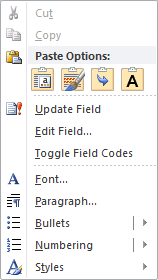
\includegraphics[width=0.20\textwidth]{meniu.png}
        \caption{Selectarea prin click dreapta a opțiunii ,,Update field''}
        \label{fig:mesh1}
    \end{figure}

    \item Selectarea opțiunii ,,Update entire tabl'' conform cu \autoref{fig:mesh2}
    \begin{figure}[h]
        \centering
        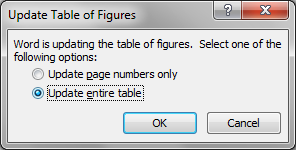
\includegraphics[width=0.35\textwidth]{meniu2.png}
        \caption{Actualizarea întregului tabel}
        \label{fig:mesh2}
    \end{figure}

    \item Verificarea fontului folosit pentru conținutul propriu-zis al Listei Tabelelor și alegerea 
    fontului Times New Roman în caz de incongruență.
    
    \begin{table}[h]
    \begin{center}
        \begin{tabular}{|c|c|c|}
            \hline\rowcolor[HTML]{f2f2f2}\textbf{Index} & \textbf{Nume utilizator} & \textbf{Valoarea rezumat a parolei (folosind SHA1)} \\\hline
            1 & dpopescu & 8fb9e6763269ae7cba85f02668c3c32041bf00ed \\\hline
            2 & eganea & 3b42ba8a586dd1589e949c28c9cf2810f7d65bb4 \\\hline
            3 & mmarian & bfc01d16d1944f3b6caba515556713f4aeeb2d0b \\\hline
        \end{tabular}
    \end{center}
    \caption{\label{tab:tabel1}\textbf{Nume de utilizatori și valorile rezumat ale parolelor acestora.}}
    \end{table}

\end{enumerate}

\newpage
În interiorul lucrării, tabelul poate fi citat folosind eticheta și numărul de ordine ale sale precum în 
exemplul acesta (vezi \autoref{tab:tabel1}). 

\subsection{Legenda (unei figuri/tabele)}
În cele doua secțiuni de mai sus s-au demonstrat două modele de legende atașate fiecărei tabele sau 
figuri. Microsoft Word permite modificarea, respectiv adăugarea de etichete noi corespunzătoare unui 
anumit tip de legendă. 

\chapter{TERMENI DE UTILIZARE}

\section{Autorii}

Acest șablon de document a fost creat de Marius Marian pentru colectivul Facultății 
de Automatică, Calculatoare și Electronică a Universității din Craiova și pentru 
uniformizarea structurii proiectelor de diplomă ale studenților săi.

\section{Licența de utilizare}

Nu există restricții de utilizare. Documentul nu este constrâns de nicio licență. 
Sugestiile de îmbunătățire pot fi adresate autorului pe adresa de e-mail: marius.marian@cs.ucv.ro.

\chapter{CONCLUZII}

Autorul prezintă concluziile sale…

\chapter{BIBLIOGRAFIE}

\begin{singlespace}
\fontsize{12}{11}\selectfont
Bibliografia va fi ordonată alfabetic dupa eticheta fiecărei element (de ex. 
DOOM05 în lista de mai jos este o etichetă). Etichetele materialelor consultate 
vor fi formatate folosind:

\begin{itemize}
    \item primele litere ale primului autor urmate de cele două cifre semnificative ale anului apariției materialului, sau
    \item dintr-un acronim popular al lucrării respective, urmat din nou de cele două cifre semnificative ale anului apariției.
\end{itemize}


[DOOM05] – \textit{Dicţionarul ortografic, ortoepic şi morfologic al limbii române}, Editura Univers Enciclopedic, Bucureşti, 2005  
\end{singlespace}


\chapter{REFERINȚE WEB}
\fontsize{12}{11}\selectfont

Recomandăm și aici respectarea regulilor enunțate pentru secțiunea 5.\\~\\

\begin{singlespace}
\fontsize{12}{11}\selectfont

[Alm08] – Pedro de Almeida, Patrik Fuhrer, Documentation Guidelines for 
Diploma and Master Thesis, Universitatea din Fribourg, Elveția, 2008, 
disponibil on-line la adresa http://diuf.unifr.ch/drupal/softeng/teaching/guidelines \\~\\

[Olt07] – Th. Olteanu, C. Albu, \textit{Ghid pentru redactarea lucrării de diplomă sau 
a disertaţiei de masterat}, Universitatea Română de Arte și Științe ,,Gheorghe Cristea'', 
2007, disponibil via web la adresa http://www.ugc.ro/tpl/GHID REDACTARE DIPLOMA LICENTA.pdf 

\end{singlespace}

\setcounter{chapter}{0}
\renewcommand{\thechapter}{\Alph{chapter}}

\chapter{CODUL SURSĂ}

În această anexă se adaugă codul sursă al aplicației…

\chapter{SITE-UL WEB AL PROIECTULUI}

Autorul prezintă în această anexă (opțională) site-ul web asociat proiectului său.

\chapter{CD / DVD}

\begin{singlespace}
    Autorul atașează în această anexă obligatorie, versiunea electronică a aplicației, 
    a acestei lucrări, precum și prezentarea finală a tezei.
\end{singlespace}

\begin{center}
    
\includegraphics{cd.png}
\end{center}

\end{document}